\documentclass[12pt]{article}
\usepackage{geometry}                % See geometry.pdf to learn the layout options. There are lots.
\geometry{letterpaper}                   % ... or a4paper or a5paper or ... 
\usepackage{graphicx}
\usepackage{amssymb}
\usepackage{amsthm}
\usepackage{epstopdf}
\usepackage[utf8]{inputenc}
\usepackage[usenames,dvipsnames]{color}
\usepackage[table]{xcolor}
\usepackage{hyperref}
\DeclareGraphicsRule{.tif}{png}{.png}{`convert #1 `dirname #1`/`basename #1 .tif`.png}

\theoremstyle{definition}
\newtheorem{example}{Example}

\newenvironment{explanation}{%
   \setlength{\parindent}{0pt}
   \itshape
   \color{blue}
}{}

\newcommand{\projectname}{Roboducks}
\newcommand{\productname}{Robo Ducks}

\newcommand{\projectleader}{Florentin Gewessler}
\newcommand{\documentstatus}{In process}
%\newcommand{\documentstatus}{Submitted}
%\newcommand{\documentstatus}{Released}
\newcommand{\version}{V. 0.1}

\begin{document}
\begin{titlepage}
\begin{flushright}

\end{flushright}

\vspace{10em}

\begin{center}
{\Huge System Specification} \\[3em]
{\LARGE \productname} \\[3em]
\end{center}

\begin{flushleft}
\begin{tabular}{|l|l|}
\hline
Project Name & \projectname \\ \hline
Project Leader & \projectleader \\ \hline
Document state & \documentstatus \\ \hline
Version & \version \\ \hline
\end{tabular}
\end{flushleft}

\end{titlepage}
\section*{Revisions}
\begin{tabular}{|l|l|l|}
\hline
\cellcolor[gray]{0.5}\textcolor{white}{Date} & \cellcolor[gray]{0.5}\textcolor{white}{Author} & \cellcolor[gray]{0.5}\textcolor{white}{Change} \\ \hline
test date&test name&test use \\ \hline
\end{tabular}
\pagebreak

\tableofcontents

\pagebreak
\section{Initial Situation and Goal}

\subsection{Initial Situation}


Our goal is to participate in the German Open Standard Platform League. The German Open Standard Platform League is a soccer league where all teams participate using the same robot, the NAO robot from SoftBank Robotics. These robots play fully autonomously and each one takes decisions separately from the others, but they still have to play as a team by using communications. The teams play on a green field with white lines and goal posts, with no other landmarks, and the ball consists in a realistic white and black soccer one. These game characteristics generate a very challenging scenario, which allows improving the league every year. Our competition are mostly teams from universities like the team B-Human which comes from the university Bremen. In this field it is very important to have sponsors because the most schools and universities can not effort too many robots. We have talked to some of the other teams and they said they would need about 50.000 Euros a year. 
As we mentioned earlier, our main goal is to participate in the German Open Standard Platform League but we can break this down to many sub goals. The first sub goal would be that we finish the framework, which we call “Duckburg”, till the 24.12.2018. The framework is the base of our software which will  contain the basic functions of a system. 


\pagebreak

\subsection{Application Domain}
Our software will be used on the NAO-Robots. With our software it will be possible that the robots play soccer in teams of five. Our software will also be optimized for the limited resources of the NAO Robots. The robots only have a ATOM Z530 singlecore CPU with 1.6 Gigahertz, 1 GB of RAM and up to 10 GB of storage. Furthermore, our software has to be very modular and expandable. This is granted through a specific system architecture which we will elaborate later in the system architecture and interfaces section.
\newline
All in all, we can summarize our project in three major steps.
The first one would be, that the Duckburg, our basic framework, is fully implemented because that is a major requirement to start further development. 
\newline
The second step would be the development of the different Engines and Agents which will do specific tasks like walking or kicking a ball. The challenges are very varied depending on which task you like to develop. For example if we want to  write an Engine and the associated agents we will have major problems with to balance of the robot but if we want to develop a Engine for recognising a ball we will have to face other problems.
\newline
The last step would be the the communication between one robot to another one. Here we have to deal with the limitations of the wlan module of the robots which allows only a small number of kilobytes between the robots. 
\newline




\pagebreak

\subsubsection{Glossary}
\begin{tabular}{|l|l|}
\hline
\cellcolor[gray]{0.5}\textcolor{white}{Fold Concept} & \cellcolor[gray]{0.5}\textcolor{white}{Description} \\ \hline
Duckburg&Basic Framework provides the basis of our system \\ \hline
Engines&Manages the agents for an specific task\\ \hline
Agents&Providing specific function like walking\\ \hline
NAO-Robots&The kind of robots we are using\\ \hline
NAO-QI&pre installed framework\\ \hline
\end{tabular}


\pagebreak
\subsubsection{Model of the Application Domain}


\subsubsection{Overview of the Business Processes}
do not exist

\subsubsection{Description of the Business Processes}

\subsection{Goal Definition}
The goal of Roboducks is to participate in the German open Standard Platform League (SPL), where 5 Naos play soccer against other teams currently there is no other team from Austria and non that is from a Higher Technical School. For archiving this goal we have to program a new framework because the existing one from Aldebaran (NaoQi) is slow and in some cases not reliable. The new framework is made with C++ which provides as language a awesome performance and memory efficiency. With the new framework we can focus on our main goal to play football with the robots and program smart techniques to play out an Universitie team which would be an great phus for our schools reputation.

\pagebreak
\section{Functional Requirements}
The system must be: lightwate in CPU and RAM usage, easy to add/remove features,  capable with several NAO generations, football……
\pagebreak
\subsection{Use Case Diagrams}
\begin{flushright}
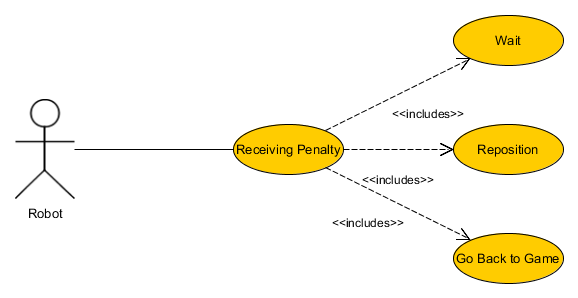
\includegraphics[scale=.5]{Penalty.png}\\
\end{flushright}
The SPL Rulebook has strict definitions for Penalties. Basically if a robot does something wrong it gets informed via the GameController and and one of the assistant referee will carry the robot to a specific spot at the sideline of the game area so that the robot cant see the game. After the penalty time the robot must turn around and and get his position to return to the game. An important thing to point out is that the penalty time increases during the game.
In general it would be good if ouer code detects/avoid forbidden actions. 

\begin{flushright}
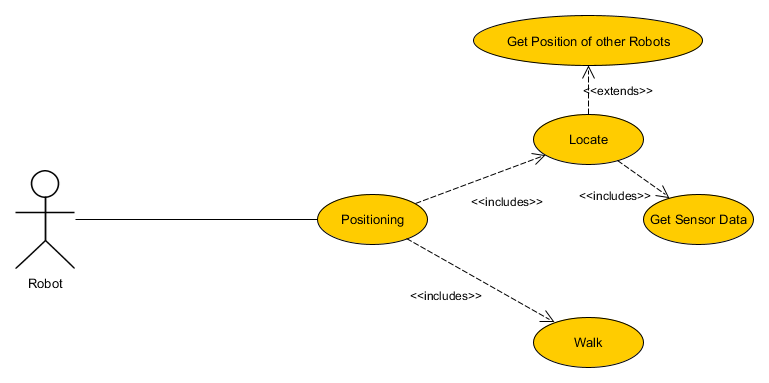
\includegraphics[scale=.5]{Positioning.png}\\
\end{flushright}
For getting the Position the Robot needs to analyse the sensor data primarily form the Cameras and maby form the infrared sensors to. The analysation is based on detecting the game aeria borders with them the robot can calculate with Trigonometry where he is. An other option is to ask the other team members where he is but for this we have to implement some smart code.


\begin{flushright}
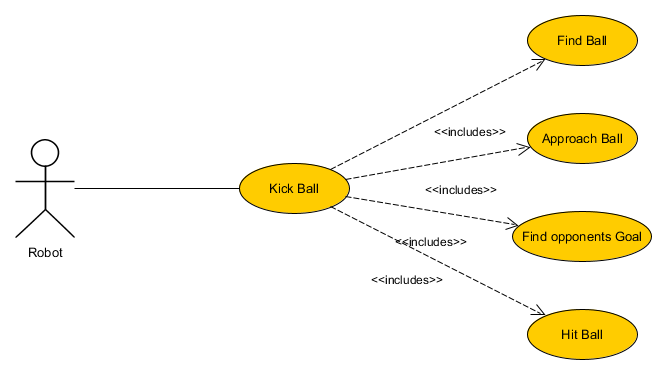
\includegraphics[scale=.5]{Kick_the_Ball.png}\\
\end{flushright}
For kicking the ball the robot must find the ball there are agan to ways a he can do it by himself or aske the other robots. Than the robot must go to the ball and gave it a hit into the ride directions.

\begin{flushright}
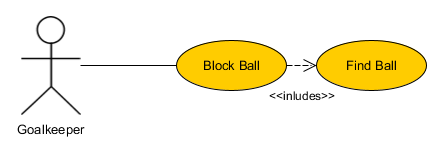
\includegraphics[scale=.5]{BlockBall.png}\\
\end{flushright}
If the ball cames to the robot with the goalkeeper role he schuld calculate where the ball might go so that he can stop it.
\pagebreak
\subsection{Use Case Details}

\pagebreak
\subsubsection{Characteristic Information}

\pagebreak
\subsubsection{GUI to call the use case}

\pagebreak
\subsubsection{GUIs for the standard use}

\pagebreak
\subsubsection{Scenarios for non-standard uses (bad cases or work around cases)}

\pagebreak
\subsubsection{GUIs for the non-standard uses}

\pagebreak
\subsubsection{Workflow}

\pagebreak
\subsubsection{Open Points}
\pagebreak
\section{Non-functional Requirements}
\pagebreak
\section{Quantity Structure}
\pagebreak
\subsection{System Architecture and Interfaces}
\pagebreak
\subsection{Acceptance Criteria}
\pagebreak
\subsection{List of Abbreviations}
\pagebreak
\subsection{References}





\end{document}  